\documentclass{beamer}

\usepackage{amsmath}
\usepackage{amssymb}
\usepackage{subfiles}
\usepackage{graphicx}
%====================================================== %
\begin{document}
%\begin{frame}
%\frametitle{Statistical Disclosure Control}
%\begin{itemize}
%\item Official Statistics
%\item Disclosure Control
%
%\item k-anonymity
%\item l-diversity
%\end{itemize}
%\end{frame}
%===================================================== %
% % GOOD
\begin{frame}
	\frametitle{Statistical Disclosure Control}
	\begin{itemize}
		\item Official Statistics and Survey Methodology
		\item Numerous Topics including:
		\item Martin Templ (Univ. of Vienna)
		\item The \textbf{sdcMicro} package
		\item (R Conference in Romania)
	\end{itemize}
\end{frame}

%====================================================== %
\begin{frame}
\frametitle{Official Statistics}
\begin{quotation}
\noindent Official statistics are statistics published by government agencies or other public bodies such as international organizations. They provide quantitative or qualitative information on all major areas of \textbf{citizens' lives}, such as economic and social development, living conditions,health, education, and the environment.\\ (Wikipedia)
\end{quotation}

\begin{itemize}
\item Remark: Are we talking about data about individual people?
\end{itemize}
\end{frame}
%====================================================== %
\begin{frame}
	\frametitle{Official Statistics}
	\begin{quotation}
"Personally identifiable information" (PII), as used in US privacy law and information security, is information that can be used on its own or with other information to identify, contact, or locate a single person, or to identify an individual in context. 
\end{quotation}
\end{frame}
%====================================================== %
\begin{frame}
\frametitle{Official Statistics}
\begin{quotation}
\noindent  PII is "any information about an individual maintained by an agency, including \\ (1) any information that can be used to distinguish or trace an individual‘s identity, such as name, social security number, date and place of birth, mother‘s maiden name, or biometric records; and \\ (2) any other information that is linked or linkable to an individual, such as medical, educational, financial, and employment information."
\end{quotation}
(NIST Special Publication 800-122)
\end{frame}

\begin{frame}
\begin{itemize}
\item 
\item \textbf{De-anonymization} is the reverse process in which anonymous data is cross-referenced with other data sources to re-identify the anonymous data source.
\end{itemize}
\end{frame}
%====================================================== %
\begin{frame}
Celebrities since 1950 (may be deceased )
\begin{itemize}
\item US, Born in 1935,  identical twin, other twin deceased.
% \item US, Bell's Palsy
\item US, Redhaired, 6"4'
\item UK, Greek Cypriot Heritage, Convert to Islam
\item UK, Female, amputation of left leg below the knee
\item Irish, Male, Blond-haired, Mullingar
\item USA, Married to UK based Lawyer.
\item UK, Same Sex Marriage, 27 years older than husband.
\item Mexican, Irish Heritage
\end{itemize}

\end{frame}


%====================================================== %
\begin{frame}
\begin{figure}
\centering

\includegraphics[width=1.1\linewidth]{./JPEGS/Slide1}
\end{figure}
\end{frame}
%====================================================== %
\begin{frame}
\begin{figure}
\centering

\includegraphics[width=1.1\linewidth]{./JPEGS/Slide2}
\end{figure}
\end{frame}
\begin{frame}
\begin{figure}
\centering
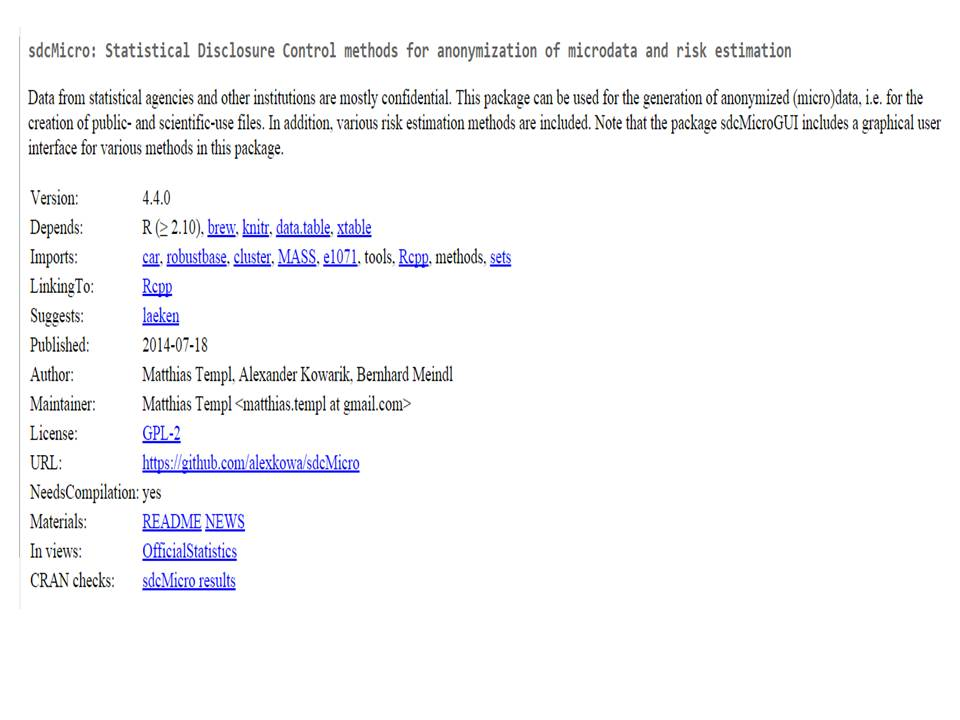
\includegraphics[width=1.1\linewidth]{./JPEGS/Slide3}

\end{figure}
\end{frame}
%====================================================== %
\begin{frame}
\begin{figure}
\centering
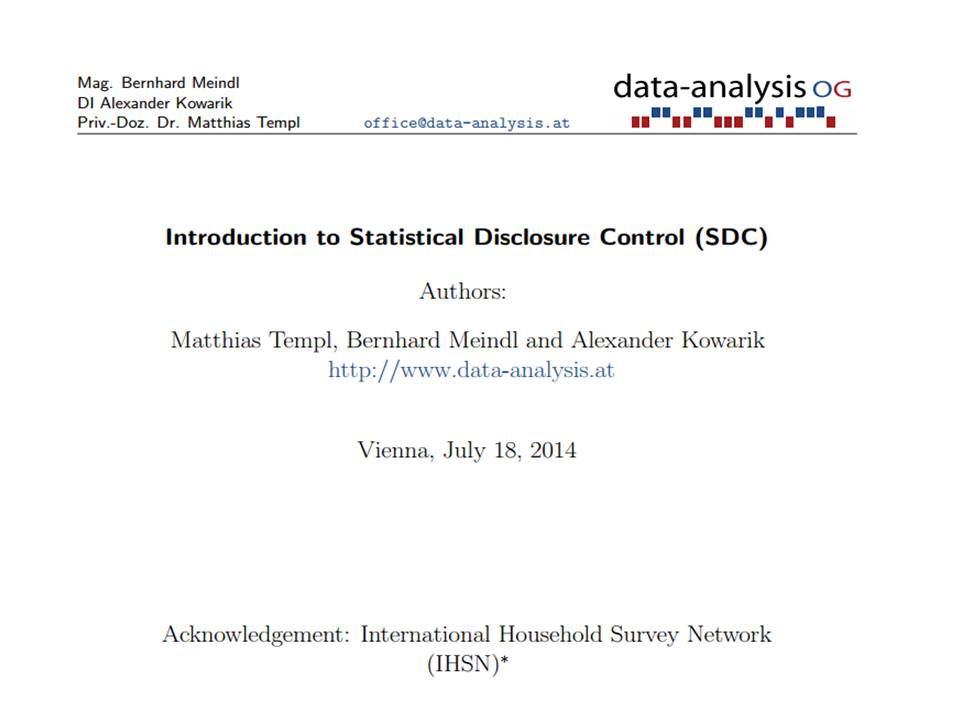
\includegraphics[width=1.1\linewidth]{./JPEGS/Slide4}
\end{figure}
\end{frame}
%====================================================== %
%\subfile{Concepts.tex}
%\subfile{IHSN.tex}
%\subfile{k-anonymity.tex}
%\subfile{sdcMicro.tex}
%\subfile{measuringrisk.tex}
%\subfile{suda.tex}
%====================================================== %
\begin{frame}
\frametitle{Statistical Disclosure Control}

\end{frame}
\end{document}
